\section{(6 points)}

La loi de financement de la Sécurité sociale comprend un objectif national de dépenses d'assurance maladie, qui est voté chaque année par le Parlement.

Le montant des dépenses d'assurance maladie a été évalué pour l'année 2016 à \num{185.2} milliards d'euros. Le parlement a voté une croissance de ces dépenses de \num{2.1} \% pour l'année 2017.

\subsection{}

\begin{questions}
	\question Montrer que le montant des dépenses  d'assurance maladie voté pour l'année 2017 est de \num{189.1} milliards d'euros \emph{(à cent millions près)}.
	
	
	
\end{questions}

\subsection{}

Pour estimer estimer les montants des années suivantes, on suppose que le Parlement votera chaque année une augmentation de \num{2.1} \% de ces dépenses.

On modélise à l'aide d'une suite $(v_n)$ le montant, en milliards d'euros des dépenses d'assurance maladie voté chaque année. On note $v_0$ le montant voté pour l'année 2016 et $v_n$ le montant voté pour l'année (2016 + $n$), où $n$ est un entier positif ou nul. On a ainsi $v_0 = \num{185.2}$.


 On veut utiliser la feuille de calcul automatisé ci-dessous afin d'obtenir les valeurs successives de la suite $(v_n)$.
 
 \begin{center}
 	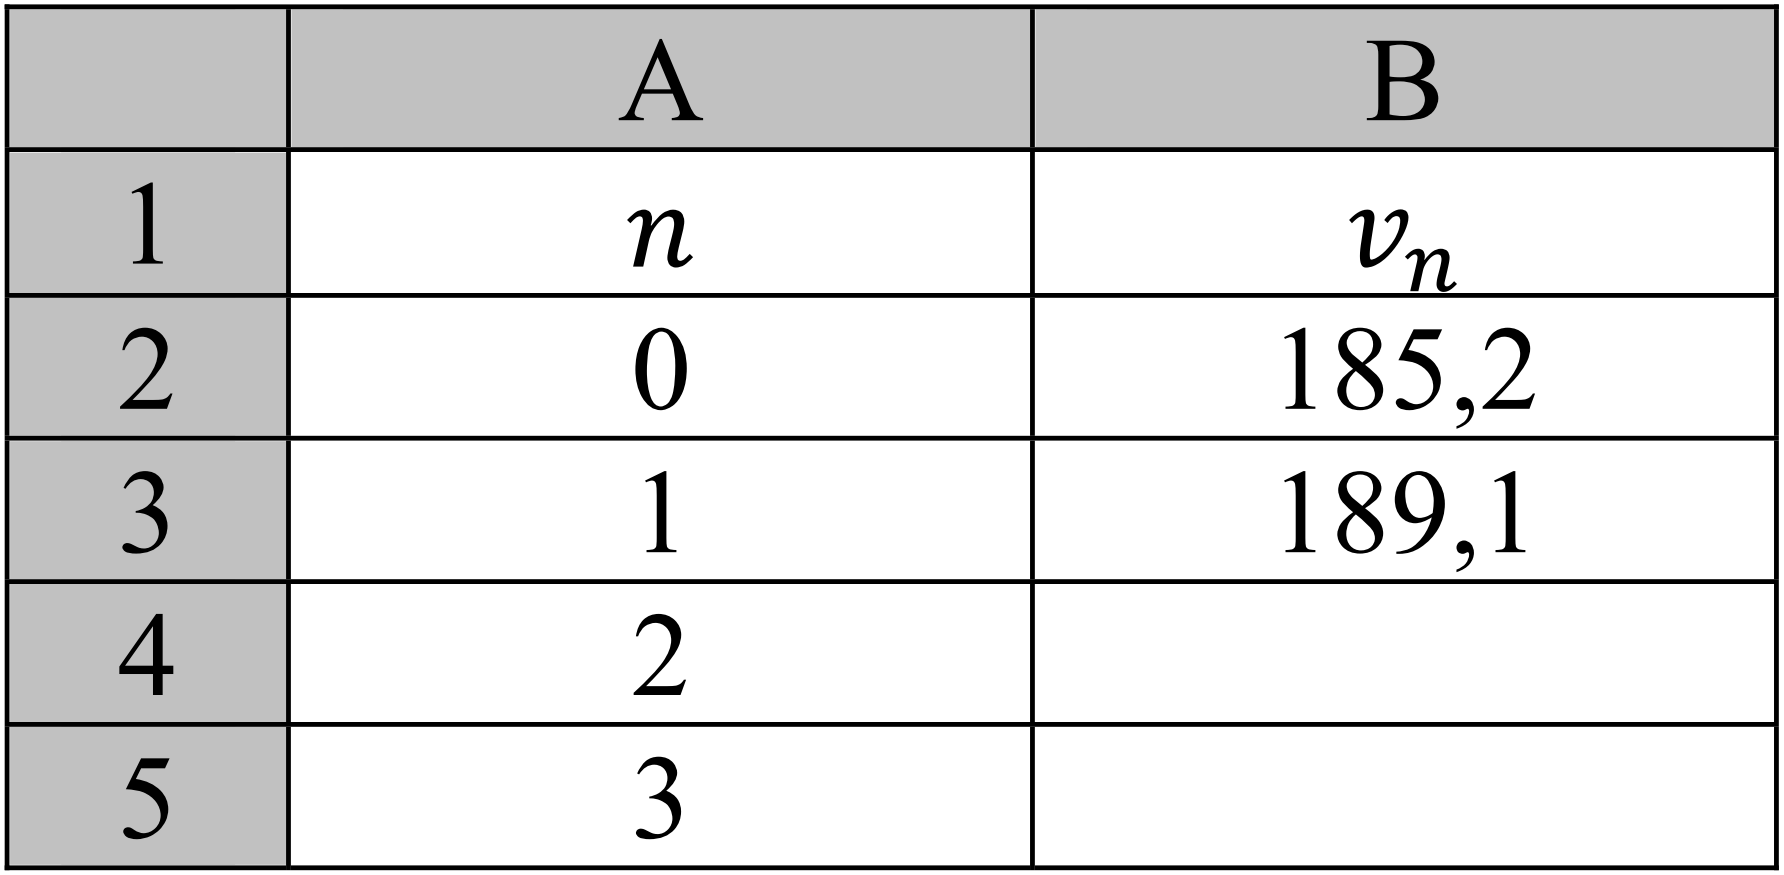
\includegraphics[scale=0.2]{img/secu}
 \end{center}

\begin{questions}
	\question Quelle formule peut-on entrer dans la cellule $B3$, de sorte que, recopiée vers le bas, elle permette d'afficher les valeurs de la suite $v_n$ ?
	\question Indiquer sans justification la nature de la suite $(v_n)$. Donner sa raison.
	
	\question Exprimer $v_n$ en fonction de $n$.
	
	\question Déterminer une estimation de montant des dépenses d'assurance maladie voté par le parlement l'année 2020. \emph{(Arrondir la valeur à la centaine de millions.)}
	
	\question \`A l'aide de la calculatrice, trouver la valeur de $x$ telle que $\num{185.2} \times \num{1.021}^x \ge \num{210}$.
	
	\question Déterminer, suivant ce modèle, l'année pour laquelle sera voté, pour la première fois, un montant de dépenses de l'assurance maladie supérieur à 210 milliards d'euros. 
\end{questions}